\documentclass[tikz,border=5pt]{standalone}
\usetikzlibrary{calc,intersections}

\begin{document}

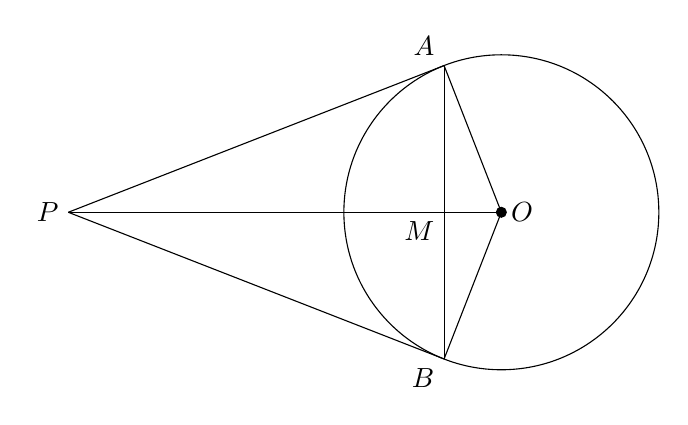
\begin{tikzpicture}[scale=1]

% Circle center and radius
\coordinate (O) at (4,0);
\def\r{2}

% External point
\coordinate (P) at (-1.5,0);

% Circle
\draw (O) circle (\r);

% ---- Compute tangent points correctly ----
\pgfmathsetmacro{\d}{veclen(4+1.5,0)} % distance PO
\pgfmathsetmacro{\angle}{acos(\r/\d)}

\coordinate (A) at ($(O)+({180-\angle}:\r)$);
\coordinate (B) at ($(O)+({180+\angle}:\r)$);

% Tangent lines
\draw (P) -- (A);
\draw (P) -- (B);

% Radii to tangent points
\draw (O) -- (A);
\draw (O) -- (B);

% Line PO
\draw (P) -- (O);

% Chord AB
\draw (A) -- (B);

\fill (O) circle (2pt);

% Intersection point M (PO with AB)
\path[name path=PO] (P) -- (O);
\path[name path=AB] (A) -- (B);
\path[name intersections={of=PO and AB, by=M}];

% Labels
\node[left] at (P) {$P$};
\node[right] at (O) {$O$};
\node[above left] at (A) {$A$};
\node[below left] at (B) {$B$};
\node[below left] at (M) {$M$};

\end{tikzpicture}

\end{document}
